
The risk methodology used in this assignment is taken from the OWASP Risk
Methodology~\cite{owasprisk} with modifications to the risk matrix.\sidenote[4.5cm]{OWASP uses a 3x3 table whereas we use a 5x5 table for better granularity.}





Risk categories are defined in table ~\ref{tab:risk_cat}.\\


Each accepted threat is given a likelihood score which is based on threat agent and vulnerability factors as well as an impact score which is based on technical impact and business impact.  These two scores are used to enter the risk matrix in figure~\ref{fig:riskmatrix} which will yield a risk category.

\begin{table}[h]
    \centering
    \begin{tabular}{l l l }
    \hline
    Risk Category & Definition \\
    \hline
    1 & Critical\\
    2 & High\\
    3 & Med-High\\
    4 & Med\\
    5 & Med-Low\\
    6 & Low \\
    \end{tabular}
    \caption{Risk Category Definitions}
    \label{tab:risk_cat}
\end{table}

\begin{table*}[ht]
    \centering
    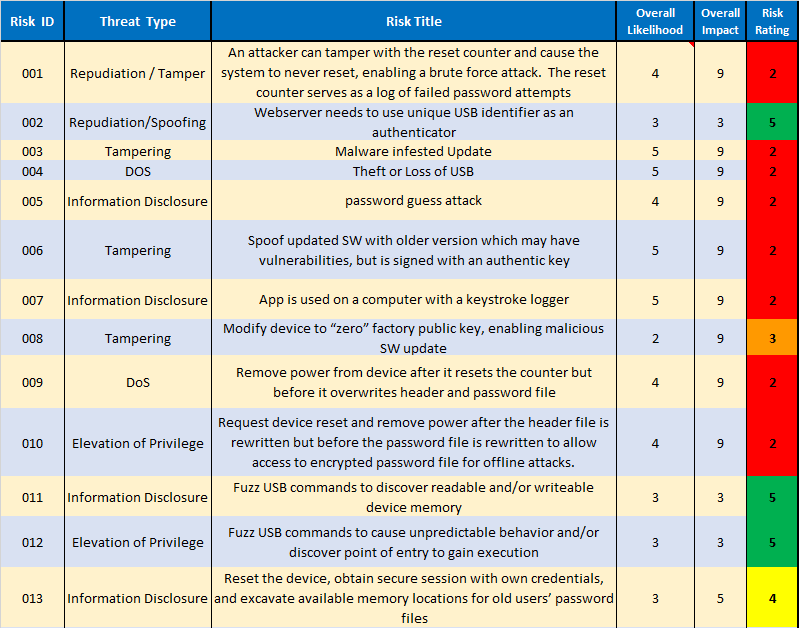
\includegraphics[width=\linewidth]{risk_sum}
    \caption{Threat Risk Summary Table}
    \label{tab:risksum}
\end{table*}


\begin{figure*}[]
    \centering
    \includegraphics[width=\linewidth]{risk_matrix}
    \caption{Populated Risk Matrix}
    \label{fig:riskmatrix}
\end{figure*}

By convention, category 1 or 2 risks require immediate attention and management
while category 5 and 6 risks can most likely be monitored.The password manager's risk are summarized using the table in table~\ref{tab:risksum}.  Detailed information concerning the factors used to asses likelihood and impact for each risk is found in table~\ref{tab:likelihood} and table~\ref{tab:impact}.



\begin{sidewaystable}[]
    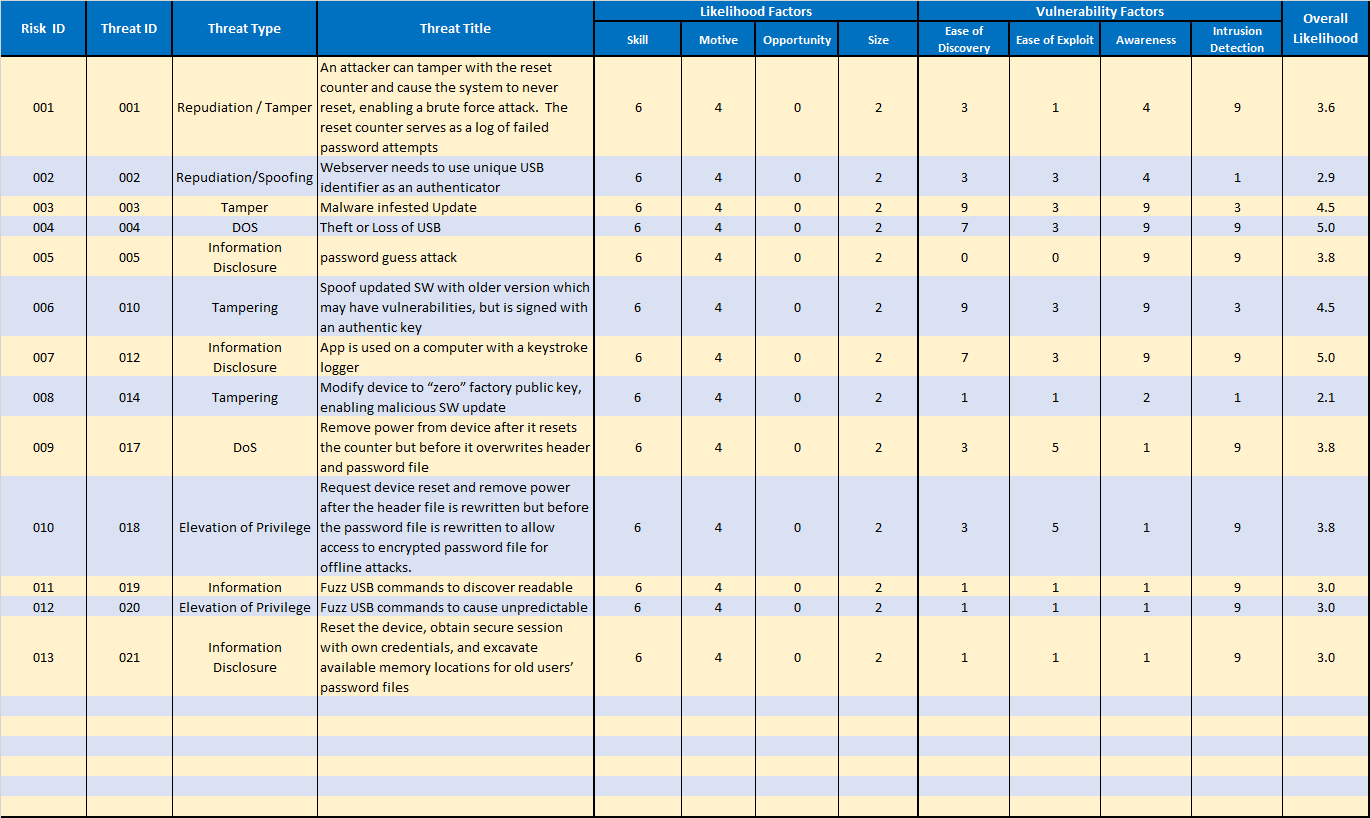
\includegraphics[]{owasp_likelihood}
    \caption{Threat Likelihood Table}
    \label{tab:likelihood}
\end{sidewaystable}

\begin{sidewaystable}[]
    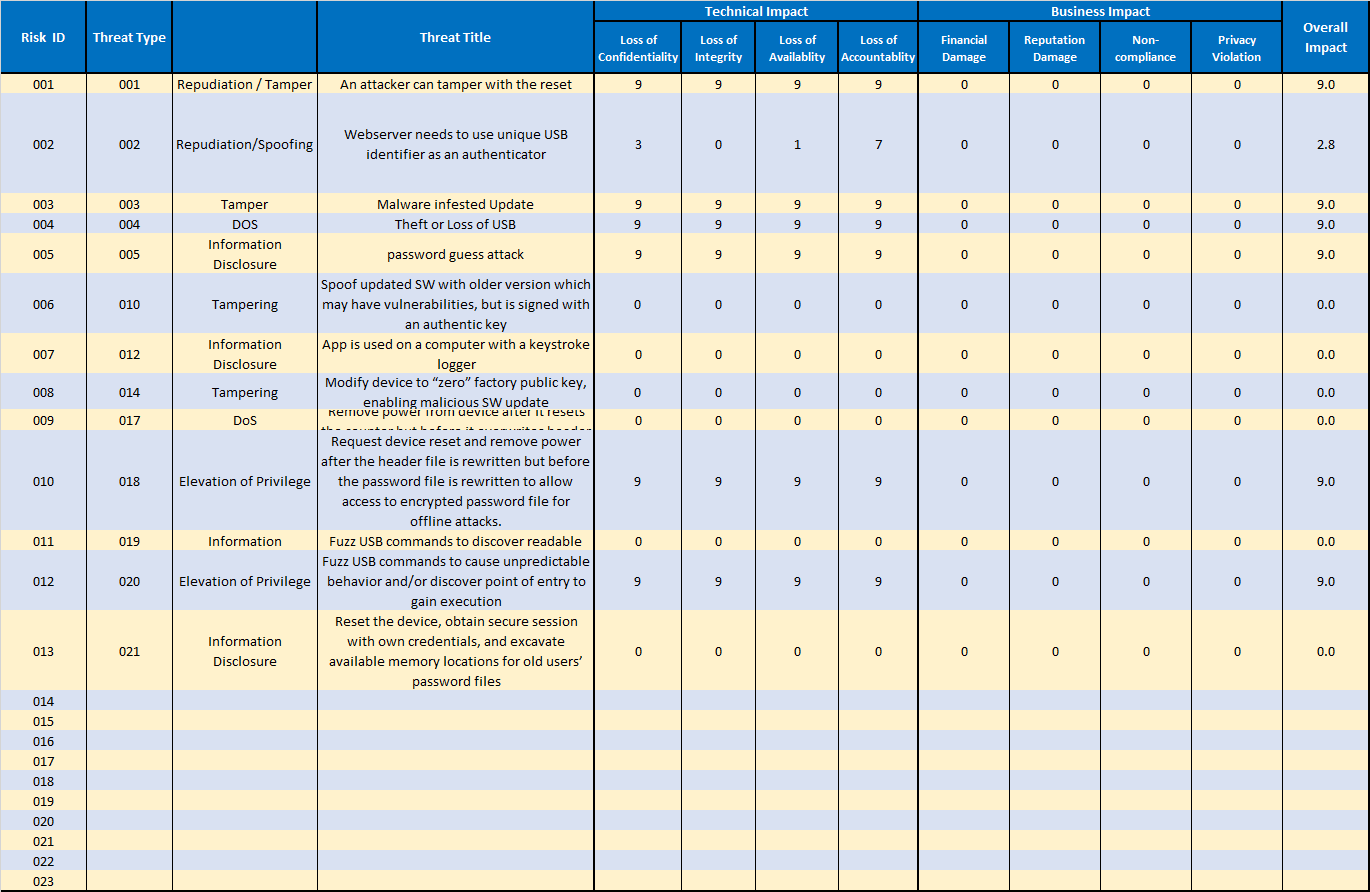
\includegraphics[]{owasp_impact}
    \caption{Threat Impact Table}
    \label{tab:impact}
\end{sidewaystable}



